\section{Zustandsregler}
\subsection{Basics}
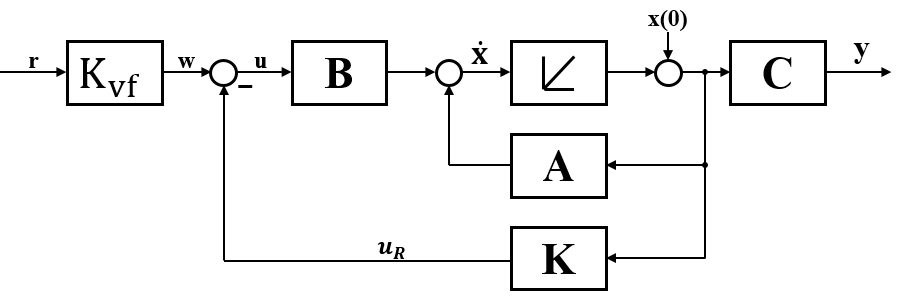
\includegraphics[width=8cm]{./bilder/regler.png}
\begin{itemize}
	\item System muss steuerbar sein, damit der Zustandsregler verwendet werden kann.
	\item Wird für die Ermittlung der fehlenden Zustände ein Beobachter gebraucht, muss das System beobachtbar sein	
	\item Der Regler besteht aus zwei Komponenten
	\begin{itemize}
		\item Feedback-Glied: $\boldsymbol{K}$ : Dieses legt die Dynamik des Reglers fest
		\item Vorwärts-Glied: $K_{vf}$ : garantiert gewünschte statische Verstärkung
	\end{itemize}
	\item Der aus Eindimensionalen Reglern bekannte Fehler $e$ gibt es nicht bei Zustandsreglern
	\item Der Zustandsregler kann auch in die in Abbildung \ref{fig:ZRD} gezeigte Zustandsraumdarstellung integriert werden
	\begin{itemize}
		\item Die Matrizen erhalten anschliessend Index $g$ 
		\item []$\boldsymbol{A}_g = \boldsymbol{A}-\boldsymbol{BK} ~~ \boldsymbol{B}_g = \boldsymbol{B}K_{vf} ~~ \boldsymbol{C}_ g = \boldsymbol{C} \hspace{5 mm}$
		\item In Gleichung \ref{eq:ss2tf} eingesetzt, kann so auch der Übergang von Übertragungsfunktion direkt zu geregeltem System gemacht werden. 
		\item [] $G(s) = \frac{Y(s)}{R(s)} = \boldsymbol{C}_g\left(s\boldsymbol{I} - \boldsymbol{A}_g\right)^{-1}\boldsymbol{B}_g
					   = \boldsymbol{C}\left(s\boldsymbol{I}-\boldsymbol{A}+\boldsymbol{BK}\right)^{-1}\boldsymbol{B}K_{vf}$
	\end{itemize}
\end{itemize}

\subsection{Polplatzierung}
\label{subsec:Polplatzierung}
\begin{figure}[!h]
	\begin{minipage}{.7\linewidth}
	\begin{itemize}
		\small
		\item Wie im Kapitel \ref{sec:ZRD} erwähnt, können Pole in eines steuerbaren Systems beliebig platziert werden
		\begin{itemize}
			\item Wenn es nicht steuerbar ist, kommt es darauf an, ob die Pole der Strecke in der positiven oder negativen Halbebene liegen. Liegen diese in der positiven Halbebene muss die Strecke modifiziert werden. Liegen diese in der negativen Halbebene muss entschieden werden ob diese so akzeptierbar sind. 
		\end{itemize}
		\item Mit dem Regler $\boldsymbol{K}$ (gleiche Dimension wie $\boldsymbol{C}$) wird das erreicht
		\item[ ] $\det\left( \lambda\boldsymbol{I}-\boldsymbol{A}+\boldsymbol{BK}\right) 
		= \left(\lambda - \lambda_1\right) \left(\lambda-\lambda_1\right)$
		\item Damit DC-Verstärkung gleich bleibt kommte der Vorfaktor $K_{vf}$ hinzu
		\item[ ] $K_{vf}=\left( \boldsymbol{C}\left( -\boldsymbol{A}+\boldsymbol{BK}\right)^{-1} \boldsymbol{B}\right)^{-1}$
		\begin{itemize}
			\item [$\Rightarrow$] Koeffizientenvergleich
		\end{itemize}
		\item Dabei soll bei der Polplatzierung folgendes beachtet werden
		\begin{itemize}
			\item Dämpfung $\xi>\frac{\sqrt{2}}{2}$ und $ \alpha = \cos^{-1}\left(\xi\right)\Rightarrow \alpha < \frac{\pi}{4}$
			\item Einschwingen schneller als $C\cdot e^{-\sigma_1}$
			\item Je schneller ein System einschwingt, desto mehr Energie benötigt es, das ist das Limit bei $\sigma_2$
			\item Der grau markierte Bereich ist anzustreben. 
		\end{itemize}
	\end{itemize}
	\end{minipage}
	\hspace{0.05\linewidth}
	\begin{minipage}[c]{.2\linewidth}
	\subfloat{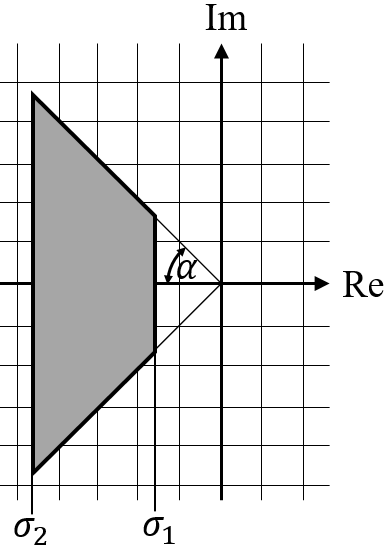
\includegraphics[width=\linewidth]{./bilder/poleLocation.png}}
	\end{minipage}
	\hfill
\end{figure}


\subsection{Optimale Regelung}
\begin{itemize}
	\item Die Kostenfunktion $J(k)$ wird als Funktion vom Regler $K$ definiert $\rightarrow J=f(K)$
	\item Durch Minimieren von $J(K)$ wird die Regelung optimiert
	\item Definition $f(K) = \int_{0}^{t_f}g(x,u) \text{dt}$ 
	\begin{itemize}
		\item  Da $x$ und $u$ von $K$ abhängig sind, ist das eine Funktion in Abhängigkeit von $K$
		\item $t_f$ bezeichnet \glqq Final Time \grqq, meist wird die als $\infty$ gewählt, da nicht der spezifische Punkt, sondern der \glqq Weg \grqq dorthin interessiert.
	\end{itemize}
	\item Für den Teil des Zustandvektors kann anstelle von $x$ auch $\vert x \vert^2$ minimiert werden
	\begin{itemize}
		\item $\vert x \vert ^2 = x^Tx$
	\end{itemize}
	\item Weiter könne einzelne Komponenten des Vektors unterschiedlich gewichtet werden, dafür wird die Matrix $\boldsymbol{Q}$ verwendet
	\item $J = \int_{0}^{\infty} x^T \boldsymbol{Q} x \text{ dt}$
	\begin{itemize}
		\item Dabei gilt, dass $\boldsymbol{Q}$ positiv semidefinit sein muss (alle Eigenwerte $\geq$ 0)
		\item Die Regelung wird zusätzlich begrenzt durch die zu Verfügung stehende Regelenergie. Siehe dazu den nächsten Abschnitt 
	\end{itemize}
\end{itemize}

\subsubsection{LQR (linear quadratischer Regler)}
\label{subsubsec:LQR}
Mit dem Hinzunehmen der möglichen Regelenergie der einzelnen Stellgrössen ergibt sich
\begin{equation*}
	J = \int_{0}^{\infty}\left(\underline{x}^T\boldsymbol{Q} \underline{x} + \underline{u}^T \boldsymbol{R} \underline{u}\right)\text{dt}
\end{equation*}
Nach dem Auflösen wird dafür folgendes Erhalten:
\begin{equation*}
	\boldsymbol{K} = \boldsymbol{R}^{-1}\boldsymbol{B}^T\boldsymbol{P}
\end{equation*}
\begin{itemize}
	\item  $\boldsymbol{P}$ aus der Gleichung \ref{eq:MatrixRiccatti}, und im Spezialfall als Skalar aus der Gleichung \ref{eq:Ricatti1D}
	\item Hierbei stammen $\boldsymbol{A}$ und $\boldsymbol{B}$ vom System und $\boldsymbol{Q}$ und $\boldsymbol{R}$ sind die Gewichtungsmatrizen
	\item Für $\boldsymbol{P}$ gibt es mehrere Lösungen, es wird die positiv definite Lösung verwendet
	\item Oftmals wird $\boldsymbol{Q} = \boldsymbol{R} = \boldsymbol{I}$ gennommen
\end{itemize}
\begin{equation}
	\label{eq:MatrixRiccatti}
	\boldsymbol{A}^T\boldsymbol{P}+\boldsymbol{PA}-\boldsymbol{PBR}^{-1}\boldsymbol{B}^T\boldsymbol{P} = -\boldsymbol{Q}
\end{equation}
\begin{equation}
	\label{eq:Ricatti1D}
	2ap-\frac{1}{r}b^2p^2+q = 0
\end{equation}

\subsubsection{Robustheit des LQR}
\begin{itemize}
	\item Für ein Singleinput-System ist eine Phasenreserve von $\pm$ \ang{60} garantiert und eine Amplitudenreserve von $\left[\right.0.5\ldots\infty\left.\right[$
	\item Für die Herleitung (Kalmann Ungleichung) und MIMO-Systeme siehe Skript \glqq State Regulator \grqq, Seite 8. 
\end{itemize}

\subsection{Zustandsregler mit intgrierendem Anteil}
\begin{figure}[h!]
	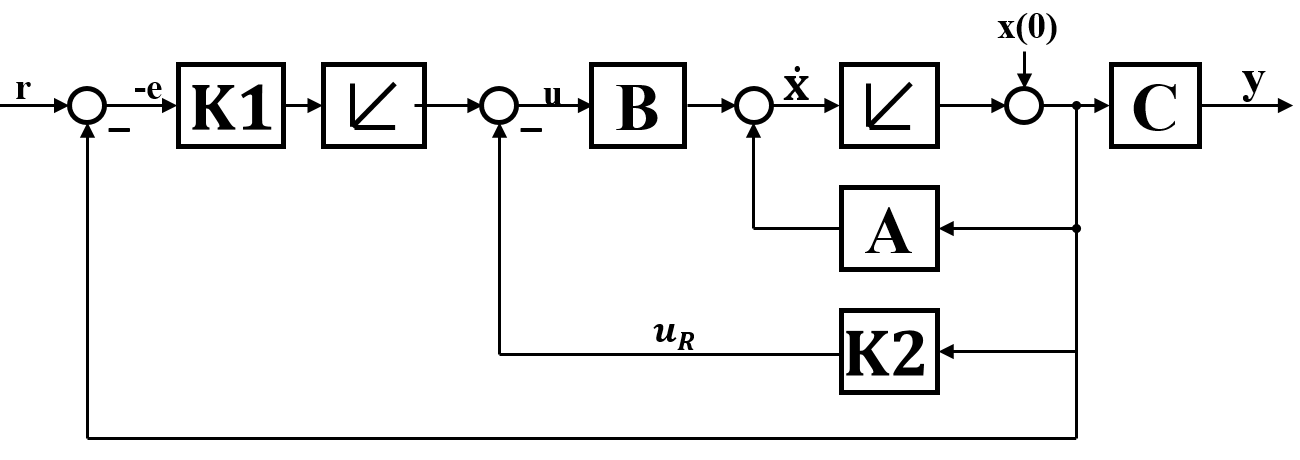
\includegraphics[width=0.5\linewidth]{bilder/zrdIntegrierend}
	\label{fig:zrdintegrierend}
\end{figure}
Zwei Möglichkeiten diesen Regler zu berechnen
\begin{itemize}
	\item[1.] Als Kaskadierten Regler
	\begin{itemize}
		\item [a)] $\boldsymbol{K2}$ mit Polplatzierung berechnen (innerer Loop)
		\item [b)] $\boldsymbol{K1}$ mit der kassischen Methode auslegen
		\item  Der Nachteil ist, dass auch eine Gute Pollage bei $\boldsymbol{K2}$ nichts nützt, wenn $\boldsymbol{K1}$ nicht gut erstellt werden kann. 
	\end{itemize}
	\item[2.] Ersatzschema für den Regler, für weitere Details siehe Skrip \glqq State Regulator \grqq, Seite 9.
	\begin{itemize}
		\item $u(t) = -K_1 \int_{0}^{t}e(\tau)\text{d}\tau-K_2x(t)$
	\end{itemize}
\end{itemize}
\newpage
